\subsection{Celkové shrnutí odevzdání}
\label{subsec:implementation-summary}

Kromě jednotlivých návrhů na konkrétních řádcích LLM modul generuje také celkové shrnutí odevzdání viditelné na \figref{fig:frontend-summary}, které poskytuje učiteli obecný pohled na kvalitu řešení.
Toto shrnutí má výhradně informativní charakter a není určeno k publikaci studentovi, proto pro něj není k dispozici akce přijetí.

Jedinou akcí u celkového shrnutí je možnost \textbf{skrytí} (\textit{dismiss}), které shrnutí skryje z pohledu učitele.
Z hlediska datového modelu je odložení shrnutí ekvivalentní zamítnutí u jednotlivých návrhů, liší se však sémanticky: zamítnutí vyjadřuje hodnotící rozhodnutí, zatímco skrytí pouze skrývá informativní obsah bez negativního hodnocení.

\begin{figure}[ht]
    \centering
    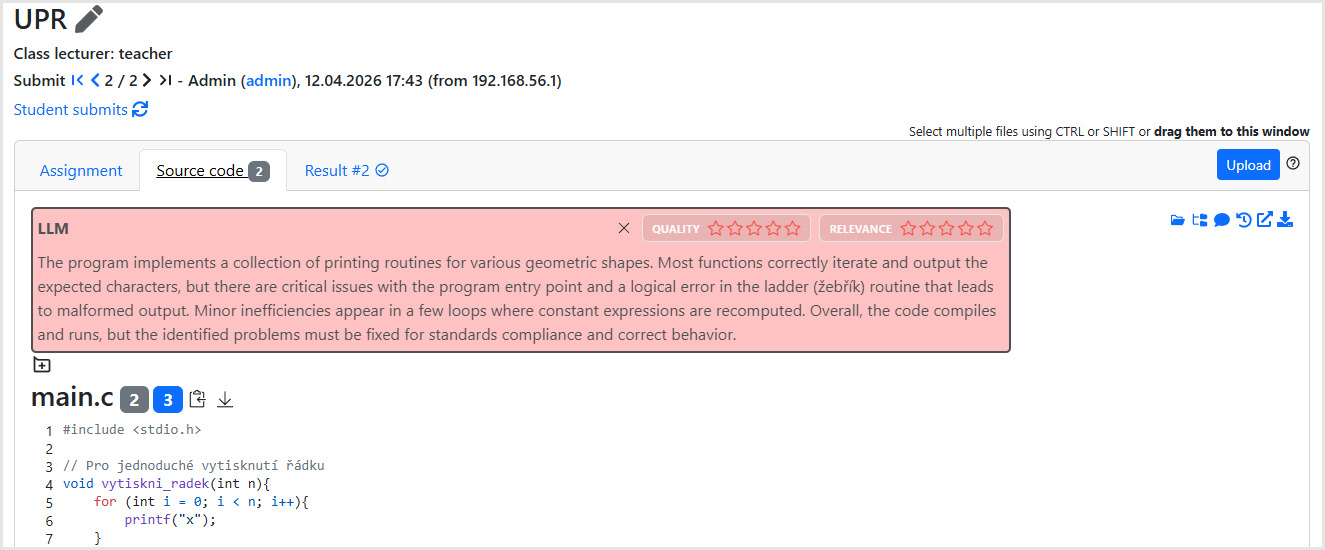
\includegraphics[width=1.0\textwidth]{resources/images/frontend-summary}
    \caption{Příklad zobrazení informativního shrnutí odevzdání v uživatelském rozhraní systému Kelvin.}
    \label{fig:frontend-summary}
\end{figure}

\endinput